
%(BEGIN_QUESTION)
% Copyright 2011, Tony R. Kuphaldt, released under the Creative Commons Attribution License (v 1.0)
% This means you may do almost anything with this work of mine, so long as you give me proper credit

Suppose this electric-driven air compressor refuses to start when the switch is in the ``Auto'' position, but starts up immediately when the switch is placed in the ``Hand'' position.  The first test performed by a technician is to measure AC voltage between test points {\bf A} and {\bf F} with the switch in the ``Auto'' position.  There, the meter registers 117 volts AC.  You are then called in to help:

$$\includegraphics[width=15.5cm]{i03458x01.eps}$$

Identify the likelihood of each specified fault for this circuit.  Consider each fault one at a time (i.e. no coincidental faults), determining whether or not each fault could independently account for {\it all} measurements and symptoms in this circuit.

% No blank lines allowed between lines of an \halign structure!
% I use comments (%) instead, so that TeX doesn't choke.

$$\vbox{\offinterlineskip
\halign{\strut
\vrule \quad\hfil # \ \hfil & 
\vrule \quad\hfil # \ \hfil & 
\vrule \quad\hfil # \ \hfil \vrule \cr
\noalign{\hrule}
%
% First row
{\bf Fault} & {\bf Possible} & {\bf Impossible} \cr
%
\noalign{\hrule}
%
% Another row
PSHH failed open &  &  \cr
%
\noalign{\hrule}
%
% Another row
PSH failed open &  &  \cr
%
\noalign{\hrule}
%
% Another row
PSL failed open &  &  \cr
%
\noalign{\hrule}
%
% Another row
``Hand'' switch position failed open &  &  \cr
%
\noalign{\hrule}
%
% Another row
``Auto'' switch position failed open &  &  \cr
%
\noalign{\hrule}
%
% Another row
OL contact failed open &  &  \cr
%
\noalign{\hrule}
%
% Another row
Auxiliary ``M'' contact failed &  &  \cr
%
\noalign{\hrule}
%
% Another row
Contactor ``M'' coil failed open &  &  \cr
%
\noalign{\hrule}
} % End of \halign 
}$$ % End of \vbox

Also, comment on whether or not the initial test between points {\bf A} and {\bf F} was a useful one (i.e. did it provide any new information to help diagnose the problem?).

\underbar{file i03458}
%(END_QUESTION)





%(BEGIN_ANSWER)

% No blank lines allowed between lines of an \halign structure!
% I use comments (%) instead, so that TeX doesn't choke.

$$\vbox{\offinterlineskip
\halign{\strut
\vrule \quad\hfil # \ \hfil & 
\vrule \quad\hfil # \ \hfil & 
\vrule \quad\hfil # \ \hfil \vrule \cr
\noalign{\hrule}
%
% First row
{\bf Fault} & {\bf Possible} & {\bf Impossible} \cr
%
\noalign{\hrule}
%
% Another row
PSHH failed open &  & $\surd$ \cr
%
\noalign{\hrule}
%
% Another row
PSH failed open & $\surd$ &  \cr
%
\noalign{\hrule}
%
% Another row
PSL failed open & $\surd$ &  \cr
%
\noalign{\hrule}
%
% Another row
``Hand'' switch position failed open &  & $\surd$ \cr
%
\noalign{\hrule}
%
% Another row
``Auto'' switch position failed open & $\surd$ &  \cr
%
\noalign{\hrule}
%
% Another row
OL contact failed open &  & $\surd$ \cr
%
\noalign{\hrule}
%
% Another row
Auxiliary ``M'' contact failed &  & $\surd$ \cr
%
\noalign{\hrule}
%
% Another row
Contactor ``M'' coil failed open &  & $\surd$ \cr
%
\noalign{\hrule}
} % End of \halign 
}$$ % End of \vbox

The initial test between points {\bf A} and {\bf F} was useless.  We already knew from the symptom of the compressor running in ``Hand'' but not in ``Auto'' that the fault must be an open, and it must lie between the Hand/Off/Auto switch and test point {\bf A} somewhere.  An open fault anywhere between points {\bf A} and {\bf F} would of course drop the full control voltage, so the measurement of 117 volts AC should come as no surprise.

%(END_ANSWER)





%(BEGIN_NOTES)

\vskip 20pt \vbox{\hrule \hbox{\strut \vrule{} {\bf Virtual Troubleshooting} \vrule} \hrule}

This question is a good candidate for a ``Virtual Troubleshooting'' exercise.  Presenting the diagram to students, you first imagine in your own mind a particular fault in the system.  Then, you present one or more symptoms of that fault (something noticeable by an operator or other user of the system).  Students then propose various diagnostic tests to perform on this system to identify the nature and location of the fault, as though they were technicians trying to troubleshoot the problem.  Your job is to tell them what the result(s) would be for each of the proposed diagnostic tests, documenting those results where all the students can see.

During and after the exercise, it is good to ask students follow-up questions such as:

\begin{itemize}
\item{} What does the result of the last diagnostic test tell you about the fault?
\item{} Suppose the results of the last diagnostic test were different.  What then would that result tell you about the fault?
\item{} Is the last diagnostic test the best one we could do?
\item{} What would be the ideal order of tests, to diagnose the problem in as few steps as possible?
\end{itemize}

%INDEX% Electronics review: AC motor control circuit
%INDEX% Process: air compressor and receiver tank

%(END_NOTES)

